Timing noise refers to small-scale structure in the timing residual which
cannot be attributed to any other source and hence cannot be modelled and
included in the timing model. The presence of timing noise indicates that we do
not have a complete picture of the neutron star: there is unmodelled physics.

Characterising timing noise is a difficult task: the exact form it takes will
depend on the order of Taylor expansion used to fit the timing parameters.
Typically pulsar astronomers truncate at $\ddot{\nu}$, but fitting to higher
orders is possible and will tend to decrease the `level' of the resulting
structure understood as timing noise. Of course using a sufficiently large
number of terms in the Taylor expansion, eventually one will fit out all of the
structure.  However, the higher order fitted coefficients do not have a proper
physical interpretation unlike the frequency and its first two derivatives
which are predicted by the electromagnetic dipole model.

To illustrate timing noise and how it can depend on the order of Taylor
expansion used, in Fig.~\ref{fig: timing noise example} we show the phase
residual remaining after fitting and removing a $3^{rd}$, $4^{th}$, and
$5^{th}$ order Taylor expansion to the Crab pulsar. In all three instances we
see a quasi-periodic structure reaching residuals up to half a cycle; higher
order have lower residuals, but the form of the structure remains consistent
between orders.  \begin{figure}[htb] \centering
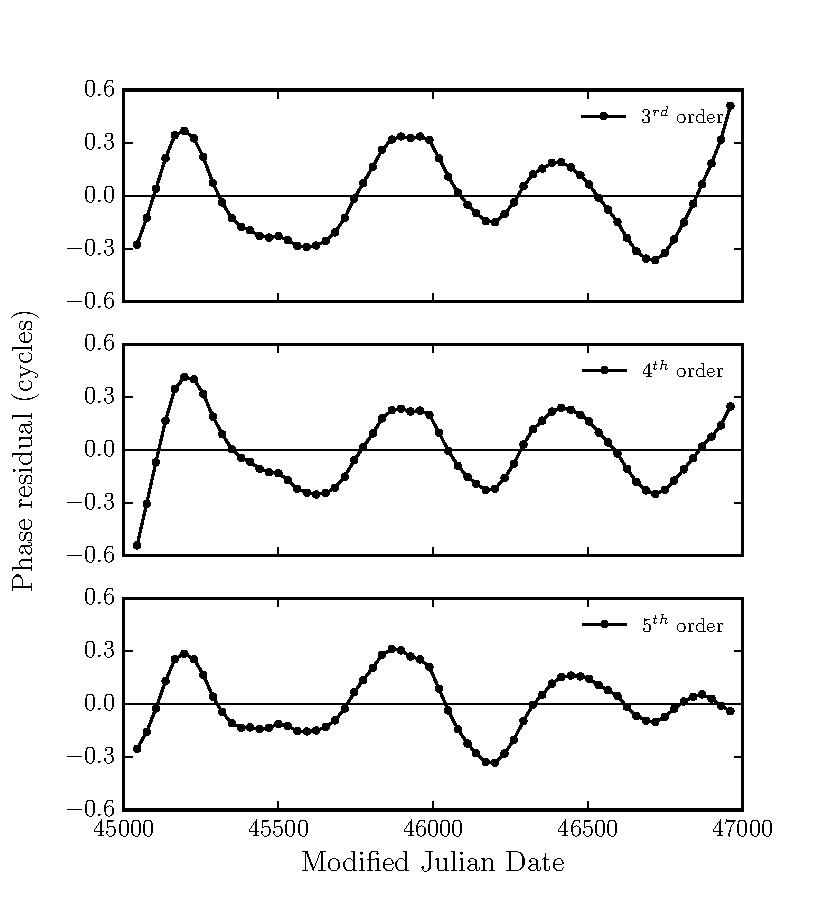
\includegraphics[width=0.75\textwidth]{PhaseResidual_45000_47000.pdf}
\caption{A phase residual demonstrating the structure which is named timing
noise. This is generated from data on the Crab pulsar (see section \ref{sec:
timing noise as described by the crab ephemeris} for details)} \label{fig:
timing noise example} \end{figure}

Several methods exist in the literature to quantify the strength of timing
noise such as the $\Delta_{8}$ value introduced by \citet{Arzoumanian1994}, the
generalisation of the Allan variance \citep{Matsakis1997}, the covariance
function of the residuals \citep{Coles2011}, and fitting for timing noise as
part of the pulsar timing model \citep{Lentati2014}.  The most comprehensive
and recent analysis was performed by \citet{Hobbs2010} who considered 366
pulsars over time scales $\gtrsim10$~years.  We summarise their conclusions
here: \begin{enumerate}

    \item Timing noise is widespread in pulsars

    \item Timing noise is inversely correlated the characteristic age defined
in equation \ref{eqn: characteristic age}

    \item The structures seen in the timing residual vary with data span: as
more data is collected, more quasi-periodic features are observed.

    \item The dominant contribution to timing noise for young pulsars with
$\tau_{c}<10^{5}$~years can be explained as being caused by the recovery from
previous glitches.

    \item A handful of pulsars exhibit significant periodicity's while
quasi-periodicity's are observed in many pulsars

\end{enumerate}

These general features give a broad picture, but there is great variation in
the form of timing noise between pulsars; this is illustrated by the variety of
timing residuals reported in \citet{Hobbs2010}. To understand the variety of
observation, in the next section we will discuss some of the models for timing
noise existing in the literature and which observations they are able to
explain.
